%-------------------------------------------------------------------------------
%                            BAB II
%               TINJAUAN PUSTAKA DAN DASAR TEORI
%-------------------------------------------------------------------------------

\chapter{TINJAUAN KEPUSTAKAAN}  

\section{Penelitian Terkait}              
Dari penelitian terdahulu, penulis tidak menemui penelitian dengan judul yang sama dengan judul penelitian penulis. Namun, penulis menemukan beberapa penelitian terkait yang dapat digunakan sebagai bahan referensi dalam menambah teori dalam penelitian ini. Tabel \ref{penelitian} adalah penelitian terkait berupa jurnal dan skripsi. 

\begin{longtable}{ |c|p{3cm}|p{4cm}|p{5cm}| }
	\caption{Penelitian terkait}
	\label{penelitian} \\
		\hline
		No & Nama Peneliti & Judul Penelitian & Hasil Penelitian \\ \hline
		\multirow{2}{*}{1.} & \citep{dadi2016} & Aplikasi Sistem Informasi Pencarian Tempat Kos di Kota Bandung Berbasis Android & Hasil dari penelitian ini adalah sebuah aplikasi yang dapat mempermudah pengguna dalam mempromosikan dan menemukan tempat penyewa yang ada di Bandung melalui Android.\\ \cline{2-4}
		& \multicolumn{3}{|p{13cm}|}{Perbedaan: Dari segi metode pengembangan sistem, penelitian yang dilakukan oleh Dadi Rosadi dan Faby Oktarista Andriawan menggunakan metode Waterfall, sedangkan penelitian penulis menggunakan metode eXtreme Programming (XP). Dari segi produk, sama-sama menghasilkan aplikasi Android tentang pencarian kos-kosan. Namun pada penelitian penulis, aplikasi yang dihasilkan bukan hanya Android tetapi aplikasi berbasis web untuk memasukkan data kos-kosan. Selain itu, penelitian ini bukan hanya pencarian kos, namun pengguna dapat melakukan pemesanan kos.} \\ \hline
		\multirow{2}{*}{2.} & \citep{hanif2013} & Pencarian Tempat Kos dengan Teknologi \textit{Augmented Reality} Berbasis Smartphone Android & Hasil dari penelitian ini adalah sebuah aplikasi yang terdiri dari aplikasi web untuk mengelola data dan aplikasi \textit{smartphone} Android yang akan digunakan sebagai alat pencarian kos. Aplikasi ini mampu menampilkan lokasi pengguna dan lokasi tempat kos terdekat di Yogyakarta dengan radius tertentu. Dengan teknologi augmented reality pada aplikasi ini pengguna dapat memperoleh informasi secara akurat dan jelas.\\ \cline{2-4}
		& \multicolumn{3}{|p{13cm}|}{Perbedaan: Dari segi produk, penelitian yang dilakukan oleh Akhmad Hanif menggunakan teknologi \textit{Augmented Reality} untuk mengetahui lokasi kos secara akurat dan jelas sedangkan pada penelitian penulis menggunakan teknologi \textit{Scan QR Code} untuk menampilkan informasi kos secara detail.} \\ \hline
\end{longtable}

\section{Kondisi Usaha Kos dan Penggunanya Saat Ini}
Berdasarkan Statistik Banda Aceh 2016, jumlah mahasiswa aktif di Universitas Negeri maupun Universitas Swasta di Aceh pada tahun 2015 mencapai 53.254 orang \citep{bappeda2016}. Dan berdasarkan Serambi Indonesia, pada tahun 2016, jumlah mahasiswa mencapai 60.838 orang. Tidak semua mahasiswa tersebut berasal dari Kota Banda Aceh sehingga mahasiswa yang merantau untuk menuntut ilmu di Kota Banda Aceh ini membutuhkan tempat tinggal yang biasa disebut dengan kos. Semakin meningkat jumlah mahasiswa, maka semakin banyak pula orang yang mencari informasi mengenai kos-kosan. Informasi tentang adanya kos-kosan biasanya dapat ditemukan pada selebaran yang ditempel di tiang listrik ataupun pohon-pohon yang ada di jalanan. Gambar \ref{selebarankos} adalah contoh selebaran pemasaran kos yang ditemui sekitar RKU Unsyiah.
 
  \begin{figure}[H]
  	\centering
  	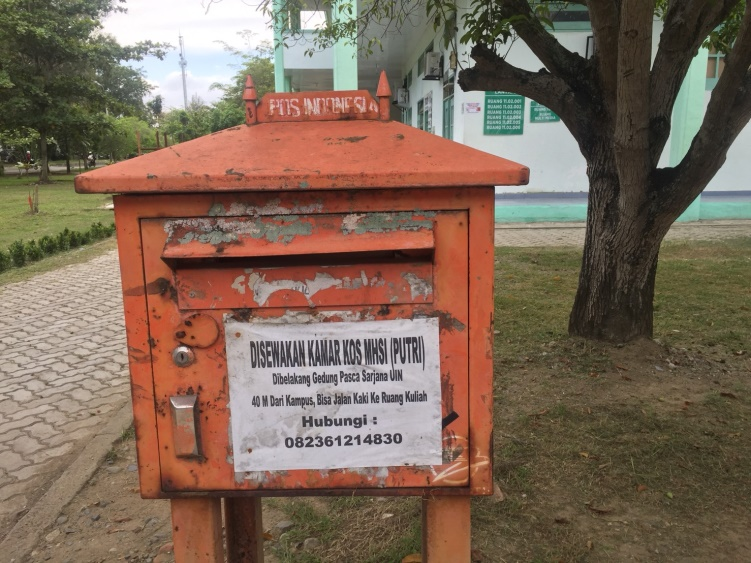
\includegraphics[scale=1.2]{gambar/selebaran}
  	\caption{Selebaran pemasaran kos.}
  	\label{selebarankos}
  \end{figure}


\section{Android}
Android merupakan sebuah sistem operasi perangkat lunak \textit{mobile} berbasis Linux yang mencakup sistem operasi, \textit{middleware} dan aplikasi \citep{supardi2011}. Android adalah \textit{platform} terbuka atau \textit{open source} sehingga siapa saja dapat membuat aplikasi berbasis Android secara gratis. Android memiliki arsitektur yang terdiri atas \textit{Applications} dan \textit{Widgets}, \textit{Applications Frameworks}, \textit{Libraries}, \textit{Android Run Time} dan \textit{Linux Kernel}. Gambar \ref{android} adalah gambaran arsitektur Android yang diambil dari website Android Developer.
  \begin{figure}[H]
	\centering
	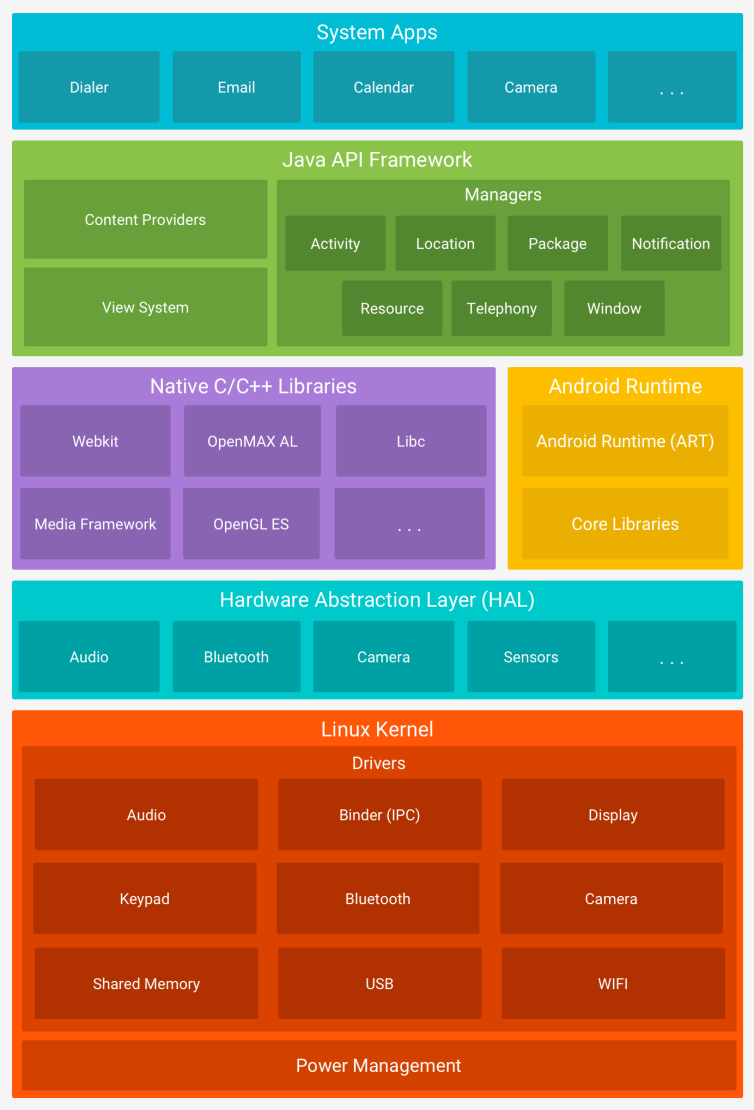
\includegraphics[scale=0.85]{gambar/android}
	\caption{Diagram Arsitektur Android.}
	\label{android}
  \end{figure}
\subsection{Kernel Linux}
Kernel Linux adalah \textit{platform} Android yang berada paling bawah. Android mengandalkan kernel Linux yang telah terbukti dengan baik untuk menyediakan fungsionalitas sistem operasinya. Kernel digunakan untuk keamanan, manajemen memori, manajemen proses, manajemen jaringan dan \textit{driver} model \citep{android2017}.

\subsection{\textit{Hardware Abstraction Layer} (HAL)}
Lapisan HAL terdiri dari beberapa modul \textit{library} yang masing-masing mengimplementasikan sebuah \textit{interface} untuk jenis komponen perangkat keras tertentu, seperti modul kamera atau Bluetooth \citep{android2017}.

\subsection{\textit{Android Runtime}}
Untuk perangkat yang menjalankan Android versi 5.0 (tingkat API 21) atau lebih tinggi, setiap aplikasi berjalan dalam prosesnya sendiri dan dengan turunannya dari \textit{Android Runtime} (ART). ART ditulis guna menjalankan beberapa mesin virtual pada perangkat bermemori rendah dengan mengeksekusi file DEX, format \textit{bytecode} yang didesain khusus untuk Android yang dioptimalkan untuk meminimalkan \textit{footprint} memori \citep{android2017}. 

\subsection{\textit{Native C/C++ Libraries}}
Android menyediakan \textit{libraries} untuk para pengembang yang menggunakan bahasa C/C++ untuk mengembangkan aplikasi Android. Jika mengembangkan aplikasi yang memerlukan kode C/C++, dapat menggunakan Android NDK (\textit{Native Development Kit}) yaitu alat yang dapat digunakan untuk mengimlementasikan aplikasi menggunakan bahasa kode asli seperti C/C++ \citep{android2017}.

\subsection{Java API Framework}
Fitur yang ada pada Android tersedia melalui API yang ditulis dalam bahasa Java. Kerangka aplikasi menyediakan kelas-kelas yang dapat digunakan untuk mengembangkan aplikasi Android \citep{android2017}. Bagian terpenting dalam kerangka aplikasi Android adalah sebagai berikut:
\begin{itemize}
	\item \textit{Activity Manager}, berfungsi untuk mengontrol siklus hidup aplikasi dan menjaga keadaan 'Backstack' untuk navigasi penggunaan.
	\item \textit{Content Providers}, berfungsi untuk merangkum data yang memungkinkan digunakan oleh aplikasi lainnya, seperti daftar nama.
	\item \textit{Resource Manager}, untuk mengatur sumber daya yang ada dalam program. Serta menyediakan akses sumber daya diluar kode program, seperti karakter, grafik, dan file layout.
	\item \textit{Location Manager}, berfungsi untuk memberikan informasi detail mengenai lokasi perangkat Android berada.
	\item \textit{Notification Manager}, mencakup berbagai macam peringatan seperti, pesan masuk, janji, dan lain sebagainya yang akan ditampilkan pada status bar.
\end{itemize}

\subsection{\textit{System Application}}
\textit{System Application} adalah aplikasi yang sudah ter-\textit{install} dalam Android. Aplikasi ini terdiri dari email, pesan SMS, kalender, \textit{browser} internet, kontak dan lainnya. Setiap perangkat dan OS Android yang berbeda, maka sistem aplikasi juga berbeda. \citep{android2017}.

\section{Kode QR (\textit{Quick Reference})}
\textit{QR (Quick Reference) Code} adalah teknologi yang muncul sebagai akibat dari keterbatasan fitur teknologi \textit{barcode linier} satu dimensi (1D), yang juga disebut sebagai kode batang klasik atau konvensional. Faktanya, penggunaan dan penerimaan teknologi kode batang sudah secara meluas di seluruh dunia karena pembacaan kode batang klasik yang cepat, akurasi dan karakteristik fungsional yang canggih. Khususnya pada sistem distribusi, telah terjadi peningkatan permintaan untuk mengkodekan data lebih dari kode batang 1D dapat menampung, terutama pada filamen seperti industri otomotif dan elektrik. Teknologi kode QR adalah teknologi yang lebih baik dengan fitur tambahan yang dirancang untuk memenuhi kebutuhan pengguna kode batang \citep{aktas2017}.

Kode batang konvensional hanya mampu menyimpan maksimal sekitar 20 digit, sedangkan kode QR mampu menangani beberapa lusin hingga beberapa ratus kali lebih banyak informasi. Kode QR mampu menangani semua jenis data, seperti karakter numerik dan abjad, Kanji, Kana, Hiragana, simbol, biner, dan kode kontrol. Hingga 7.089 karakter dapat dikodekan dalam satu simbol \citep{wave2017}. Gambar \ref{qrcode} adalah contoh dari kode QR yang menampung banyaknya karakter.

\begin{figure}[H]
	\centering
	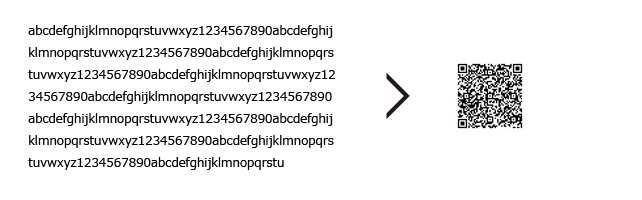
\includegraphics[width=\linewidth]{gambar/qrcode}
	\caption{Contoh kode QR.}
	\label{qrcode}
\end{figure}

Kode QR memiliki kemampuan koreksi kesalahan untuk mengembalikan data jika kode tersebut kotor atau rusak. Empat tingkat koreksi kesalahan tersedia bagi pengguna untuk memilih sesuai dengan lingkungan operasi. Peningkatan level ini meningkatkan kemampuan koreksi kesalahan namun juga meningkatkan jumlah data ukuran kode QR \citep{wave2017}. Tabel \ref{contoh1} merupakan tabel kapasitas koreksi \textit{error} pada kode QR.

\begin{table}[H]
	\centering
	\caption{Kapasitas koreksi \textit{error} kode QR}
	\label{contoh1}
	\begin{tabular}{ |l|l| }
		\hline
		Level & Koreksi \textit{Error} \\ \hline
		L & 7\% \\ \hline
		M & 15\% \\ \hline
		Q & 25\% \\ \hline
		H & 30\% \\ \hline	
	\end{tabular}
\end{table}

Data yang dapat dikodekan (\textit{generate}) menjadi kode QR adalah numerik, gambar, teks, email, kartu nama, serta situs web (URL). Data yang sudah menjadi kode QR dapat dipindai dengan menggunakan \textit{smartphone} yang sudah tersedia aplikasi pembaca kode QR. Untuk memindai kode QR, cukup membuka aplikasi dan tunggu sampai kamera mendeteksi secara otomatis. Dalam beberapa detik konten yang dikodekan ditayangkan di layar.
%-----------------------------------------------------------------------------%

\section{Basis Data}

Basis data adalah kumpulan dari data yang saling berhubungan yang dapat disusun dan dikelola sedemikian rupa agar dapat dimanfaatkan kembali dengan cepat dan mudah \citep{yanto2016}. Lingkup terbesar yang ada pada organisasi data adalah sistem basis data. Sistem basis data mencakup semua bentuk komponen data yang ada dalam suatu sistem. Sedangkan basis data adalah komponen utama yang menyusun sistem basis data \citep{pamungkas2017}. Tingkatan data dapat disusun ke dalam sebuah hierarki, mulai dari yang paling sederhana hingga yang paling kompleks. Alat untuk merancang basis data yang sering digunakan adalah \textit{Entity Relationship Diagram} (ERD). ERD adalah alat analis untuk memetakan data yang akan disimpan dalam sistem basis data. Menurut \citep{bagui2012} terdapat 3 langkah dalam siklus kehidupan rekayasa perangkat lunak untuk desain basis data, yaitu:
\begin{enumerate}[a.]
	\item Langkah pertama: Mendapatkan kebutuhan untuk basis data
	
	Pada langkah ini, pengembang akan mendengarkan dan menanyakan pertanyaan mengenai fakta (data) apa yang diinginkan oleh pengguna untuk diatur ke dalam sistem basis data.
	
	\item Langkah kedua: Spesifikasikan basis data
	
	Langkah kedua melibatkan diagram dari apa yang analis pikirkan kemauan pengguna. Desain basis data biasanya selesai dengan ERD yang berfungsi sebagai \textit{blueprint} untuk basis data yang akan dirancang. \textit{Blueprint} adalah keluaran dari langkah desain.
	
	\item Langkah ketiga: Desain Basis data
	
	Setelah basis data digambarkan dan disepakati, ERD menjadi \textit{blueprint} terakhir untuk pembangunan basis data pada langkah ketiga.
\end{enumerate}

\section{Metode eXtreme Programming}
Metode \textit{eXtreme Programming} (XP) yang dipelopori oleh Kent Beck, Ron Jeffries dan Ward Cunningham adalah salah satu metode pengembangan perangkat lunak \textit{Agile}. XP paling banyak digunakan untuk pengembangan perangkat lunak cepat karena merupakan suatu pendekatan yang ringan \citep{pressman2010}.
 
XP mencakup seperangkat aturan dan praktik-praktik yang terjadi dalam konteks empat kegiatan kerangka kerja yaitu perencanaan, perancangan, pengkodean dan pengujian. Berikut adalah ilustrasi proses XP dan penjelasan setiap proses tersebut. Gambar \ref{xp} adalah proses dari XP.

\begin{figure}[H]
	\centering
	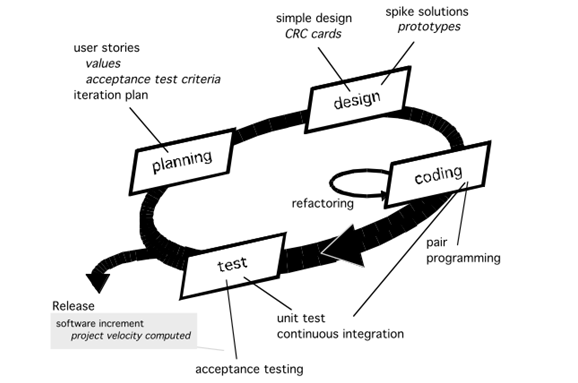
\includegraphics[width=\linewidth]{gambar/xp}
	\caption{Proses \textit{eXtreme Programming} (XP) }
	\label{xp}
\end{figure}

\begin{enumerate}[a.]
	\item \textit{Planning} (Perencanaan)
	
	Tahap perencanaan ini dimulai dengan mengumpulkan kebutuhan-kebutuhan untuk aplikasi yang akan dikembangkan dalam bentuk cerita (\textit{user stories}). \textit{User stories} menggambarkan keluaran yang diperlukan, fitur-fitur dan fungsionalitas-fungsionalitas aplikasi.
	
	\item \textit{Design} (Perancangan)
	
	Sebuah hasil perancangan yang sederhana selalu lebih disukai daripada gambaran-gambaran yang lebih kompleks. Contohnya perancangan suatu cerita akan diimplementasikan sesuai cerita tersebut, tidak kurang dan tidak lebih. Tidak disarankan untuk membuat rancangan-rancangan dan fungsionalitas-fungsionalitas tambahan (karena pengembang menganggap nantinya akan diperlukan). XP mendorong penggunaan kartu CRC (\textit{Class Responsibility Collaborator}) sebagai mekanisme yang efektif untuk berpikir tentang perangkat lunak dalam konteks berorientasi objek.
	
	\item \textit{Coding} (Pengkodean)
	
	Setelah cerita yang didapatkan dan dikembangkan dari tahap perencanaan dan perancangan, tim XP tidak langsung beralih ke kode-kode program, tetapi akan dilakukan serangkaian unit pengujian yang menjalankan setiap cerita. Setelah unit pengujian dibuat, pengembang akan lebih mampu berkonsentrasi pada apa yang harus diimplementasikan supaya lulus dari unit pengujian tersebut.
	
	\item \textit{Testing} (Pengujian)
	
	Uji kelayakan XP berfokus pada fitur-fitur dan fungsionalitas sistem/ perangkat lunak, sering disebut uji pengguna, dirinci oleh para pengguna. Pengujian ini secara keseluruhan dapat dilihat dan ditinjau kembali oleh para pengguna. Uji kelayakan berasal dari cerita pengguna yang telah diimplementasikan.
\end{enumerate}

\section{\textit{Web Service}}
\textit{Web service} adalah aplikasi klien dan \textit{server} yang berkomunikasi melalui \textit{World Wide Web} (WWW) dan \textit{HyperText Transfer Protocol} (HTTP). Seperti yang dijelaskan oleh \textit{World Wide Web Consortium} (W3C), \textit{web service} menyediakan sarana standar untuk interoperatif antara aplikasi perangkat lunak yang berjalan pada berbagai \textit{platform} dan kerangka kerja \citep{oracle2018}. Jenis \textit{web service} dapat dibagi menjadi 2 yaitu REST dan SOAP. Pada penelitian ini menggunakan \textit{web service} REST.

REST (\textit{Representational State Transfer}) diperkenalkan dan didefinisikan pada tahun 2000 oleh Roy Fielding dalam disertasi doktoralnya. Gaya arsitektur REST adalah arsitektur server klien di mana klien mengirim permintaan ke server yang menyediakan \textit{resource} kemudian server memproses permintaan dan mengembalikan respons untuk penggunaan selanjutnya \citep{mumbaikar2013}. \textit{Resource} adalah sesuatu yang diidentifikasi oleh URI.  Untuk mengakses \textit{resource} menggunakan HTTP (Hypertext Transfer Protocol) sebagai protocol untuk komunikasi data. Berikut metode HTTP yang umum digunakan dalam arsitektur berbasis REST:
\begin{enumerate}[a.]
	\item GET, mengambil informasi. Permintaan GET harus aman dan idempoten, artinya berapa pun operasi dijalankan dengan parameter yang sama, hasilnya akan tetap sama. 
	\item POST, meminta agar sumber daya di URI (\textit{Uniform Resource Identifier}) melakukan sesuatu dengan entitas yang disediakan. Selain membuat entitas baru, POST juga dapat digunakan untuk memperbarui entitas.
	\item PUT, simpan entitas di URI. PUT dapat membuat entitas baru atau memperbarui yang sudah ada. Permintaan PUT bersifat idempoten.
	\item DELETE, meminta agar sumber daya dihapus.
	\item PATCH, perbarui hanya bidang entitas yang ditentukan di URI. Permintaan PATCH bersifat idempoten. 
\end{enumerate}

\section{\textit{Problem-based Analysis}}
\textit{Problem-based analysis} adalah menganalisa sesuatu berdasarkan masalah. Sebagai dasar dari menganalisa masalah, digunakanlah pendekatan \textit{problem frames} berdasarkan penelitian Zave dan Jackson. Rekayasa kebutuhan berkaitan dengan mendeskripsikan masalah yang harus dipecahkan perangkat lunak dengan cara yang tepat. Masalah tersebut berada dalam lingkungan dimana mesin akan diintegrasi \citep{cheng2007}. Zave dan Jackson mendefinisikan tiga istilah yaitu \textit{requirements} (R), \textit{domain knowledge} (D) dan \textit{specification} (S). \textit{Requirement} menjelaskan sistem yang diinginkan setelah mesin dibangun. \textit{Domain knowledge} menggambarkan bagian yang relevan dari masalah yang ada di dunia. Dan \textit{specification} menggambarkan perilaku mesin agar memenuhi kebutuhan.

\textit{Problem frames} mendukung pengembang dalam menganalisa masalah yang harus dipecahkan \citep{beckers2014}. \textit{Problem frames} mengklasifikasikan, menggambarkan, menganalisis dan menata masalah pengembangan perangkat lunak.  Keseluruhan masalah perangkat lunak akan diuraikan menjadi sub masalah yang sederhana. Setiap sub masalah berhubungan dengan satu atau lebih kebutuhan. Solusi dari sub masalah akan disusun untuk memecahkan keseluruhan masalah perangkat lunak. Analisa kebutuhan ini sangat penting untuk menghindari modifikasi di kemudian hari dalam siklus pengembangan perangkat lunak dan untuk meningkatkan kualitas perangkat lunak secara keseluruhan \citep{alebrahim2014}. 

Menurut \citep{jackson2001} terdapat lima \textit{problem frames} dasar, yaitu:

\begin{itemize}
	\item \textit{Required behaviour}
	\item \textit{Commanded behaviour}
	\item \textit{Information display}
	\item \textit{Simple workpieces}
	\item \textit{Transformation}
\end{itemize}

Gambar \ref{pf} adalah salah satu contoh \textit{problem frames} yaitu \textit{commanded behavior}.

\begin{figure}[H]
	\centering
	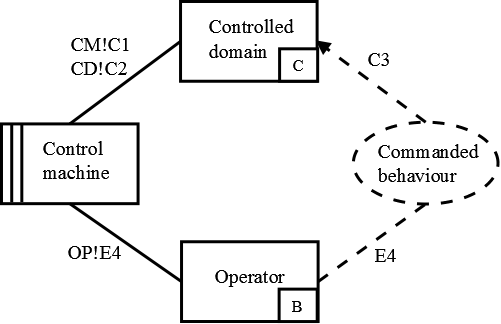
\includegraphics[scale=0.4]{gambar/pf}
	\caption{Kerangka \textit{commanded behavior}. }
	\label{pf}
\end{figure}

Komponen \textit{problem frames} mewakili hal-hal yang ada di dunia nyata:

\begin{itemize}
	\item \textit{Control machine}, yaitu perangkat lunak yang akan dibangun.
	\item \textit{Controlled domain} atau domain yang dikendalikan adalah bagian dunia yang bisa dikendalikan. Ini adalah domain \textit{causal} (peralatan mekanik atau listrik), ditandai C dalam diagram, fenomenanya bersifat fisik dan hubungan \textit{causal}. 
	\item Operator mengeluarkan perintah, Operator adalah domain \textit{biddable}, ditandai dengan B dalam diagram. 
	\item \textit{Commanded behaviour} atau perilaku yang diperintahkan adalah \textit{required behaviour} atau perilaku yang dibutuhkan dari domain yang dikontrol sebagai respons terhadap perintah operator, E4. Perilaku yang dibutuhkan ini dinyatakan dalam bentuk fenomena C3, yang pada umumnya berbeda dari C1 dan C2.
\end{itemize}
	
Selain \textit{causal} dan \textit{bidabble}, terdapat domain \textit{lexsical} yaitu representasi fisik data. Sifat \textit{lexsical} memungkinkan data untuk ditulis dan dibaca, ditandai X dalam diagram \citep{jackson2001}. 

\section{OCL (\textit{Object Constraint Language})}
\textit{Object Constraint Language} (OCL) adalah sebuah bahasa formal yang digunakan untuk menggambarkan ekspresi dan batasan yang rumit pada model UML \citep{cabot2014}. Ekspresi OCL dapat digunakan untuk menentukan operasi/tindakan yang bila dijalankan, apakah mengubah keadaan sistem atau menentukan batasan spesifik sistem. Konsep utama pada OCL adalah objek, \textit{object navigation}, \textit{collections}, \textit{collection operations} dan \textit{boolean-valued expression} serta rumus \citep{balaban2016}. Berikut penjelasan dari konsep utama OCL:

\begin{enumerate}[a.]
	\item Objek, sebuah ekspresi OCL akan sering dimulai dengan objek literal atau variabel objek dan menunjukkan nilai, objek atau kumpulan dari entitas-entitas. Contohnya p:Paper dan r:Research, p dan r adalah objek dari kelas Paper dan Research.
	\item Object Navigation, direalisasikan dengan menggunakan nama peran (role) dari asosiasi atau atribut yang bernilai objek.
	\item \textit{Collections}, dapat digunakan untuk menggabungkan elemen yang berbeda ke dalam struktur tunggal yang mengandung elemen. Ada empat jenis \textit{collections} yaitu \textit{sets}, \textit{bags}, \textit{sequences }dan \textit{ordered sets}.
	\item Collection operations, ada sejumlah operasi pengumpulan yang berkontribusi pada fleksibilitas OCL. \textit{Collection operations }biasa diterapkan dengan menggunakan operator panah. Contohnya adalah isEmpty, notEmpty, size, select, reject dan lain-lain.
	\item \textit{Boolean-valued expressions}, sering digunakan untuk mendeskripsikan kelas invarian dan operasi \textit{pre} dan \textit{post conditions}. Contohnya adalah \textit{and}, \textit{or}, \textit{not}, =, \textit{implies}, \textit{xor}, \textit{forAll }dan \textit{exist}. 	
\end{enumerate}

\textit{Constraint} (kendala) dalam OCL harus dirumuskan pada tingkat kelas dan dalam konteks kelas tertentu. Ada tiga jenis \textit{constraint}: \textit{invariant}, \textit{postcondition} dan \textit{precondition}. \textit{Invariant} (inv) adalah \textit{constraint} yang menyatakan apabila operasi dijalankan, kondisi harus selalu benar. \textit{Precondition} harus benar sebelum operasi dijalankan sedangkan \textit{postcondition} harus benar sesudah operasi dijalankan. 

Kendala-kendala yang ada pada diagram UML, seperti diagram kelas sering digambarkan dalam bahasa alami. Praktik telah menunjukkan bahwa ini akan selalu menghasilkan ambiguitas. Untuk menulis kendala yang tidak ambigu, dapat menggunakan bahasa formal. Kelemahan dari bahasa formal tradisional adalah bahwa hal itu dapat digunakan untuk orang-orang dengan latar belakang matematis yang kuat, namun sulit bagi perancang bisnis atau yang bukan berlatar belakang matematis. Sehingga OCL digunakan untuk menerjemahkan  diagram kelas menjadi bahasa formal yang mudah dibaca dan ditulis.

\section{UML Diagram Kelas}
UML adalah bahasa standar untuk pemodelan aplikasi berorientasi objek dan umumnya digunakan dalam pengembangan aplikasi perangkat lunak. UML dikembangkan terutama untuk desain perangkat lunak, bagian utama dari desain perangkat lunak melibatkan perancangan basis data yang akan diakses oleh modul perangkat lunak. Oleh karena itu, bagian penting dari UML adalah diagram kelas. Diagram kelas adalah jenis diagram yang menggambarkan struktur statis sistem dengan menunjukkan kelas sistem dan hubungan di antara keduanya \citep{soler2010}. Contoh UML Diagram Kelas dapat dilihat pada gambar \ref{diagkelas}.

\begin{figure}[H]
	\centering
	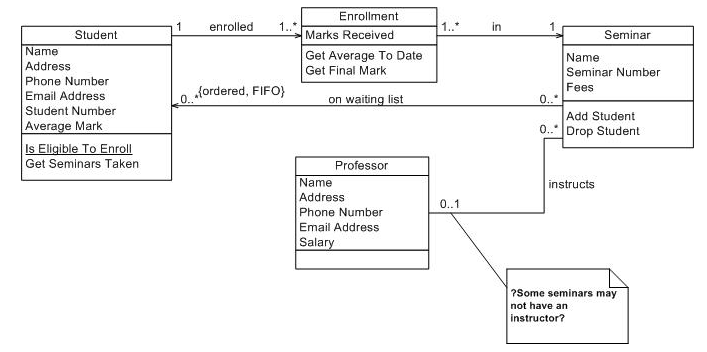
\includegraphics[width=\linewidth]{gambar/diagramkelas}
	\caption{Contoh diagram kelas }
	\label{diagkelas}
\end{figure}

\begin{itemize}
	\item Kelas, adalah representasi dari sebuah objek dan, dalam banyak hal, ini hanyalah sebuah template dari objek yang diciptakan. Pada Gambar 2.6 yaitu \textit{Student}, \textit{Enrollment}, Profesor, dan Seminar.
	\item Asosiasi, menunjukkan bahwa kelas tersebut merujuk kepada sebuah objek atau lebih dari satu objek dari kelas lain. Contohnya adalah "\textit{Professor instructs Seminar}".
	\item Agregasi, jenis asosiasi yang lebih kuat dan digunakan untuk mengindikasikan bahwa sebuah kelas memiliki namun juga mungkin berbagi objek dengan kelas lainnya.
	\item Pewarisan (\textit{inheritance}), "adalah" dan "seperti" hubungan, memungkinkan untuk menggunakan kembali data dan kode yang ada dengan mudah. Ketika A mewarisi dari B, A adalah \textit{subclass} dari B dan B adalah \textit{superclass} A. Notasi pemodelan UML untuk pewarisan adalah sebuah garis dengan panah tertutup menunjuk dari \textit{subclass} ke \textit{superclass}.
\end{itemize}

\section{\textit{System Usability Scale}}
\textit{System Usability Scale }(SUS) adalah sebuah metode yang dapat diandalkan untuk mengukur kegunaan (\textit{usability}) \citep{brook1996}. SUS terdiri dari 10 item kuesioner dengan lima pilihan untuk responden mulai dari Sangat Setuju sampai Sangat Tidak Setuju. Metode SUS ini tidak memerlukan jumlah sampel yang besar sehingga tidak memerlukan biaya dan waktu yang besar. SUS dapat digunakan untuk mengevaluasi berbagai macam produk dan layanan, termasuk perangkat keras, perangkat lunak, perangkat seluler, situs web dan aplikasi.
Manfaat menggunakan SUS adalah sebagai berikut:
\begin{enumerate}[a.]
	\item SUS menggunakan skala Likert yang sangat mudah untuk diberikan kepada responden.
	\item Dapat digunakan pada ukuran sampel yang kecil namun dengan hasil yang dapat diandalkan.
	\item Valid, dapat membedakan secara efektif antara sistem yang dapat digunakan atau yang tidak dapat digunakan.
\end{enumerate}

Pertanyaan dari SUS dapat dilihat pada tabel \ref{kuesioner}.

	\begin{longtable}{ |c|p{6cm}|c|c|c|c|c| }
		\caption{Daftar Pertanyaan Kuesioner SUS}
		\label{kuesioner} \\ 
		\hline
		No. & Pertanyaan & 1 & 2 & 3 & 4 & 5 \\
		\hline
		1. & Saya sepertinya akan sering menggunakan aplikasi ini. & & & & & \\
		\hline
		2.  & Saya melihat ada bagian fitur aplikasi ini yang cukup merepotkan, yang mestinya hal itu tidak perlu terjadi.
		& & & & &\\
		\hline
		3. & Saya rasa aplikasi ini mudah digunakan. & & & & & \\
		\hline
		4. & Saya sepertinya akan membutuhkan bantuan seorang teknisi agar bisa lancar menggunakan aplikasi ini.
		& & & & & \\
		\hline
		5. & Saya rasa fitur-fitur aplikasi ini sudah terintegrasi dengan baik satu sama lain.
		& & & & & \\
		\hline
		6. & Saya menemukan terlalu banyak ketidak konsistenan dalam aplikasi ini.
		& & & & & \\
		\hline
		7. & Saya pikir orang-orang akan sangat cepat bisa menggunakan aplikasi ini.
		& & & & & \\
		\hline
		8. & Saya rasa aplikasi ini sangat sulit untuk digunakan. & & & & & \\
		\hline
		9. & Saya merasa mantap menggunakan aplikasi ini.  & & & & & \\
		\hline
		10. & Saya mesti belajar banyak hal terlebih dahulu sebelum mulai menggunakan aplikasi ini
		.
		& & & & & \\
		\hline
	\end{longtable}
Keterangan : 
\\ 1 = Sangat Tidak Setuju
\\ 2 = Tidak Setuju
\\ 3 = Netral
\\ 4 = Setuju
\\ 5 = Sangat Setuju

 Cara menghitung nilai SUS adalah sebagai berikut:
\begin{enumerate}[a.]
	\item  Untuk pernyataan ganjil: skala yang diberikan responden dikurangi satu.
	\item Untuk pernyataan genap: lima dikurangi skala yang diberikan responden.
	\item Skala Sangat Tidak Setuju sampai Sangat Setuju bernilai 0 sampai 4.
	\item Jumlahkan skala responden yang telah dikonversi dan kalikan jumlahnya dengan 2,5. Ini mengkonversi rentang nilai menjadi antara 0-100. Nilai tersebut bukanlah persen.
\end{enumerate}

Untuk menentukan \textit{grade} hasil penilaian ada 2 (dua) cara
yang dapat digunakan (Brooke, 2013). Penentuan pertama dilihat dari sisi tingkat penerimaan pengguna, \textit{grade scale} dan \textit{adjective rating}. Penerimaan pengguna terdiri dari 3 kategori yaitu \textit{not acceptable}, \textit{marginal} dan \textit{acceptable}. Sedangkan dari sisi tingkat \textit{grade scale} terdapat enam skala yaitu A, B, C, D, E dan F. Dan
dari \textit{adjective rating} terdiri dari \textit{worst imaginable},
\textit{poor}, \textit{ok}, \textit{good}, \textit{excellent} dan \textit{best imaginable}. Gambar \ref{susScore2} adalah skor SUS.
\begin{figure}[H]
	\centering
	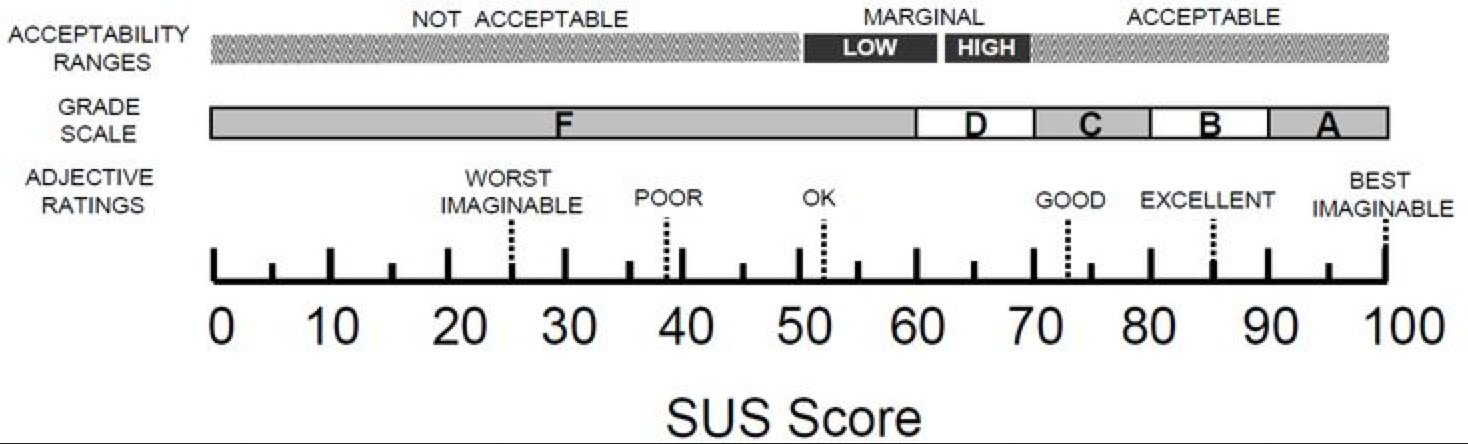
\includegraphics[width=\textwidth]{gambar/susscore}
	\caption{\textit{Grade rankings} skor SUS \citep{bangor2009}}
	\label{susScore2}
\end{figure}
Penentuan yang kedua dilihat dari sisi \textit{percentile range } yang memiliki \textit{grade} penilaian yang terdiri dari A, B, C, D dan F. 

\begin{figure}[H]
	\centering
	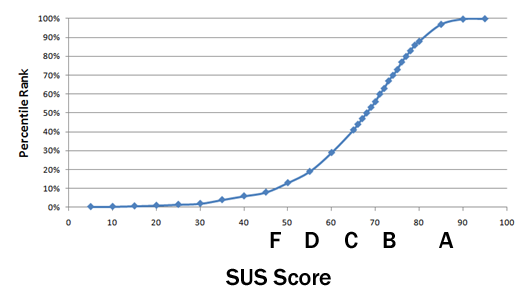
\includegraphics[width=\textwidth]{gambar/pr}
	\caption{\textit{Grade rankings} skor SUS \citep{sauro2011}}
	\label{pr}
\end{figure}

\section{Pengujian \textit{Black Box}}
Menurut \citep{pressman2010}, \textit{black box testing }berfokus pada persyaratan fungsional perangkat lunak yang memungkinkan \textit{engineers} untuk memperoleh set kondisi input yang sepenuhnya akan melaksanakan persyaratan fungsional untuk sebuah program. Pengujian \textit{black box} membantu dalam verifikasi fungsionalitas keseluruhan dari sistem yang diuji. Pengujian ini mencoba untuk menemukan kesalahan dalam kategori berikut.

\begin{enumerate}[a.]
	\item Fungsi tidak benar atau hilang.
	\item Kesalahan \textit{interface} (antarmuka).
	\item Kesalahan dalam struktur data atau akses database eksternal.
	\item Kesalahan kinerja atau perilaku.
	\item Kesalahan inisialisasi dan terminasi.
\end{enumerate}

Konsep pengujian black box yang paling sederhana adalah memeriksa spesifikasi program dan memilih kasus uji yang menjalankan semua fungsi yang terlihat secara eksternal. Ketika memilih tes black box ini, penguji mempertimbangkan tujuan program, apa yang akan di-\textit{input} dan \textit{output} yang diharapkan serta kemungkinan dimana program yang mungkin gagal \citep{thomas2002}. 


\section{Pengujian Espresso}
Espresso adalah pengujian Android yang disediakan oleh Google. Espresso didasarkan pada peningkatan Instrumentation Test Runner yang disebut Google Intrumentation Test Runner untuk membuat otomatitasi tes Android agar lebih dapat diandalkan dan lebih cepat \citep{knott2015}. Pengujian Espresso dalam \textit{Android Testing Support Library} menyediakan API untuk menulis pengujian \textit{User Interface} (UI) guna menyimulasikan interaksi pengguna dalam satu aplikasi. Pengujian Espresso berjalan pada perangkat sesungguhnya atau emulator dan berperilaku seolah-olah pengguna sesungguhnya sedang menggunakan aplikasi. Manfaat dari pengujian Espresso adalah dapat memantau semua interaksi sistem yang dimiliki aplikasi Android serta secara otomatis menyinkronkan tindakan pengujian dengan UI aplikasi. 

Contoh penggunaan Espresso adalah menemukan tombol, klik tombol dan mengecek keluaran dari tombol tersebut \cite{blundell2015}. Selain itu, pengujian ini dapat digunakan untuk sentuh, \textit{scroll} dan beberapa event lainnya. Beberapa kelas yang ada pada Espresso adalah sebagai berikut:
\begin{enumerate}
	\item ViewMatcher, berfungsi untuk mendapatkan \textit{object view} jika di \textit{activity} terdapat findViewById.
	\item ViewAction, berfungsi untuk melakukan perintah \textit{click}, \textit{scroll}, \textit{input text} dan \textit{action view} lainnya.
	\item ViewAssertion, berfungsi untuk mendapatkan hasil dari tes yang telah dilakukan.
\end{enumerate}

Berikut adalah contoh \textit{code snippet} dari pengujian Espresso:
\lstset{language=Java,
	basicstyle=\ttfamily\scriptsize\color{black},
	keywordstyle=\color{javapurple}\bfseries,
	stringstyle=\color{javared},
	commentstyle=\color{javagreen},
	morecomment=[s][\color{javadocblue}]{/**}{*/},
	numbers=left,
	numberstyle=\tiny\color{black},
	showstringspaces=false,
	numbersep=10pt,
	tabsize=4,
	showspaces=false,
	showstringspaces=false,
	autogobble=true,
	xleftmargin=2em
}

\begin{lstlisting}
@Test
public void greeterSaysHello() {
   onView(withId(R.id.name_field)).perform(typeText("Steve"));
   onView(withId(R.id.greet_button)).perform(click());
   onView(withText("Hello Steve!")).check(matches(isDisplayed()));
}
\end{lstlisting}
\captionof{lstlisting}{\textit{Code snippet} dari pengujian Espresso}




%-----------------------------------------------------------------------------%

% Baris ini digunakan untuk membantu dalam melakukan sitasi
% Karena diapit dengan comment, maka baris ini akan diabaikan
% oleh compiler LaTeX.
\begin{comment}
\bibliography{daftar-pustaka}
\end{comment}
